\chapter{\SB{} v1 Design}
\label{design}

An ideal tensegrity system, either robotic or static, is a collection of rigid compressible elements suspended within a network of tensioned cables where none of the compressible elements are in direct contact with one another. 
For robotic tensegrities without a payload, the actuation and supporting electronics would be logically designed into the compressible elements. 
For the inception of \SB{}, this compressible element called a struct was further dissected into three parts: two identical ends called Modular Tensegrity Robots (MTR) and a section of tube stock connecting the MTRs.
Connecting six of these struts into an icosahedron geometric pattern will create \SB{}.
Modular Tensgrity Robot is a loose label given to the self-contained robotic element which when connected with multiple MTRs may make up a tensegrity robot.
The current version of a MTR can be seen in figure \ref{fig:fully_assembled_endcap} and the following subsections will explain the mechanical and electrical make up of an MTR.

\begin{figure}[thpb]
\begin{subfigure}{.5\textwidth}
      \centering
      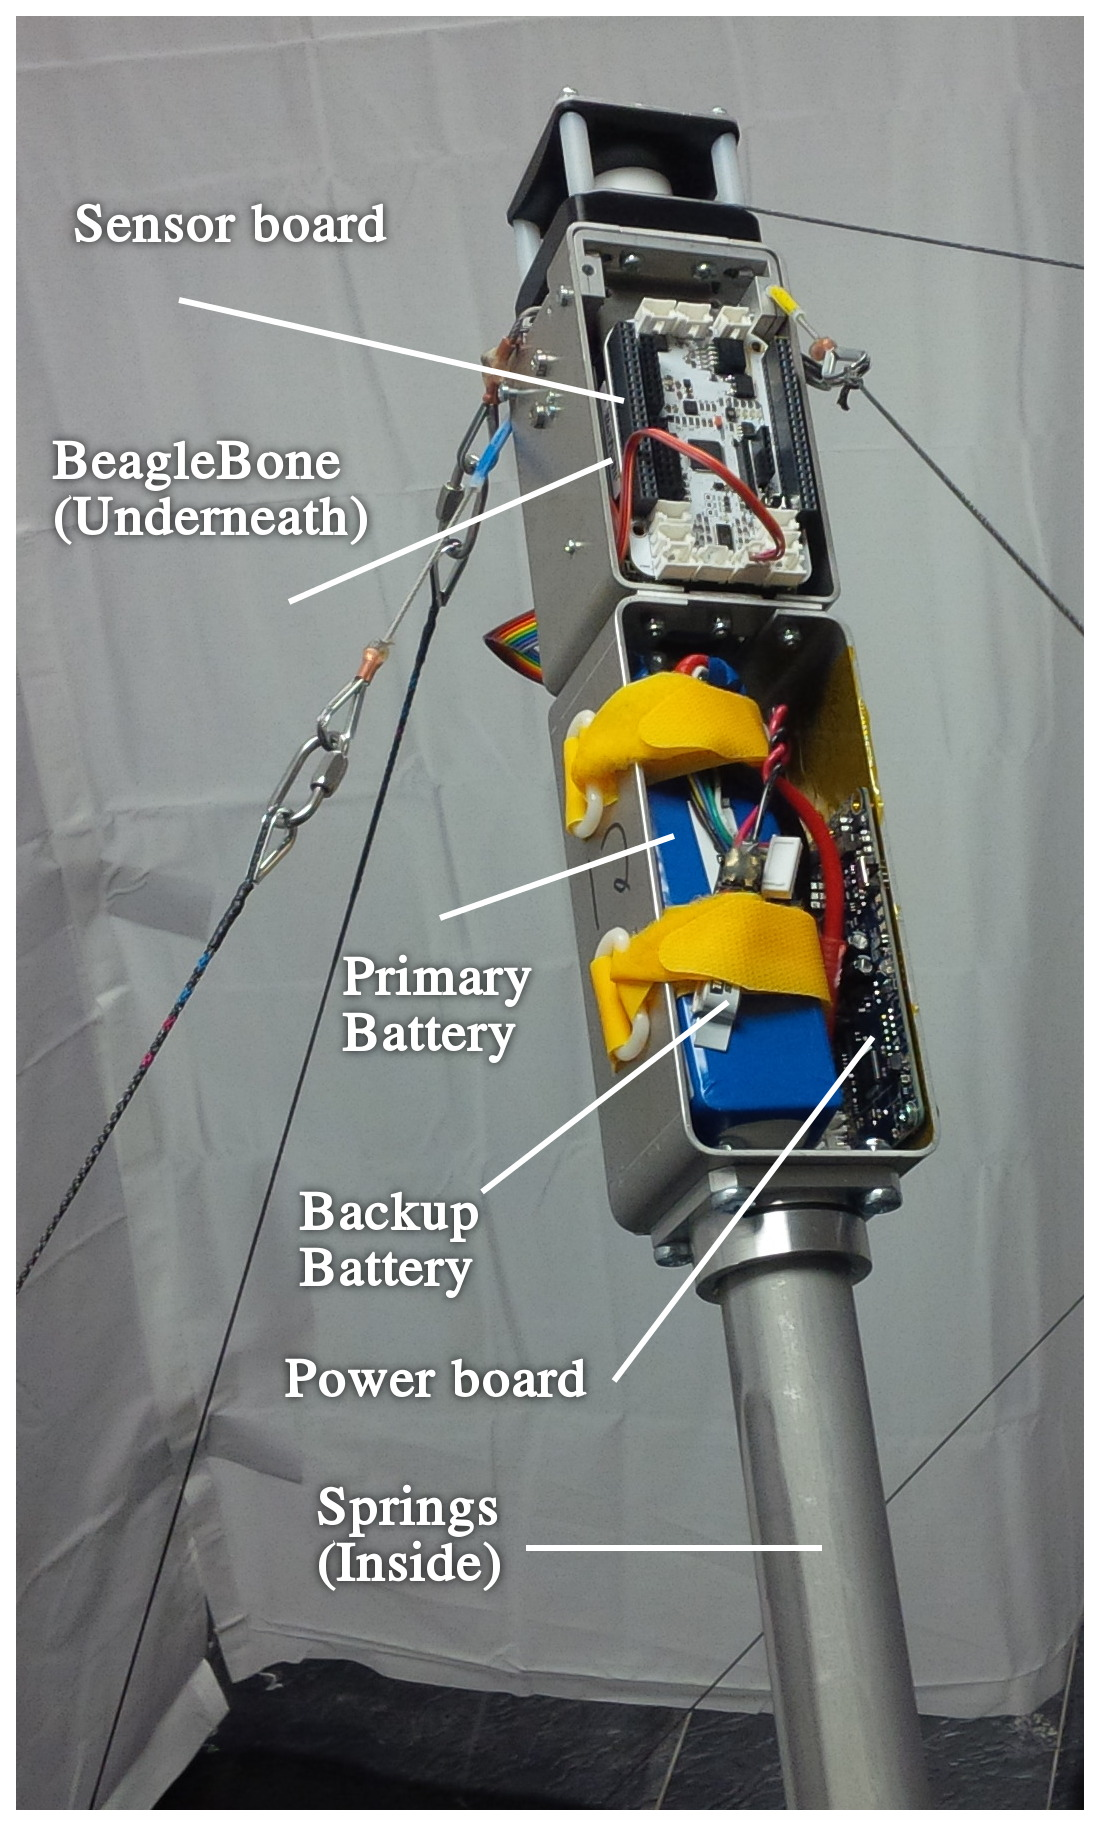
\includegraphics[width=0.5\columnwidth]{tex/img/endcap_upclose_sensorboard_labelled_fixedfonts}
      \caption{MTR front side.}
      \label{fig:endcap_upclose_front}
\end{subfigure}
\begin{subfigure}{.5\textwidth}
      \centering
      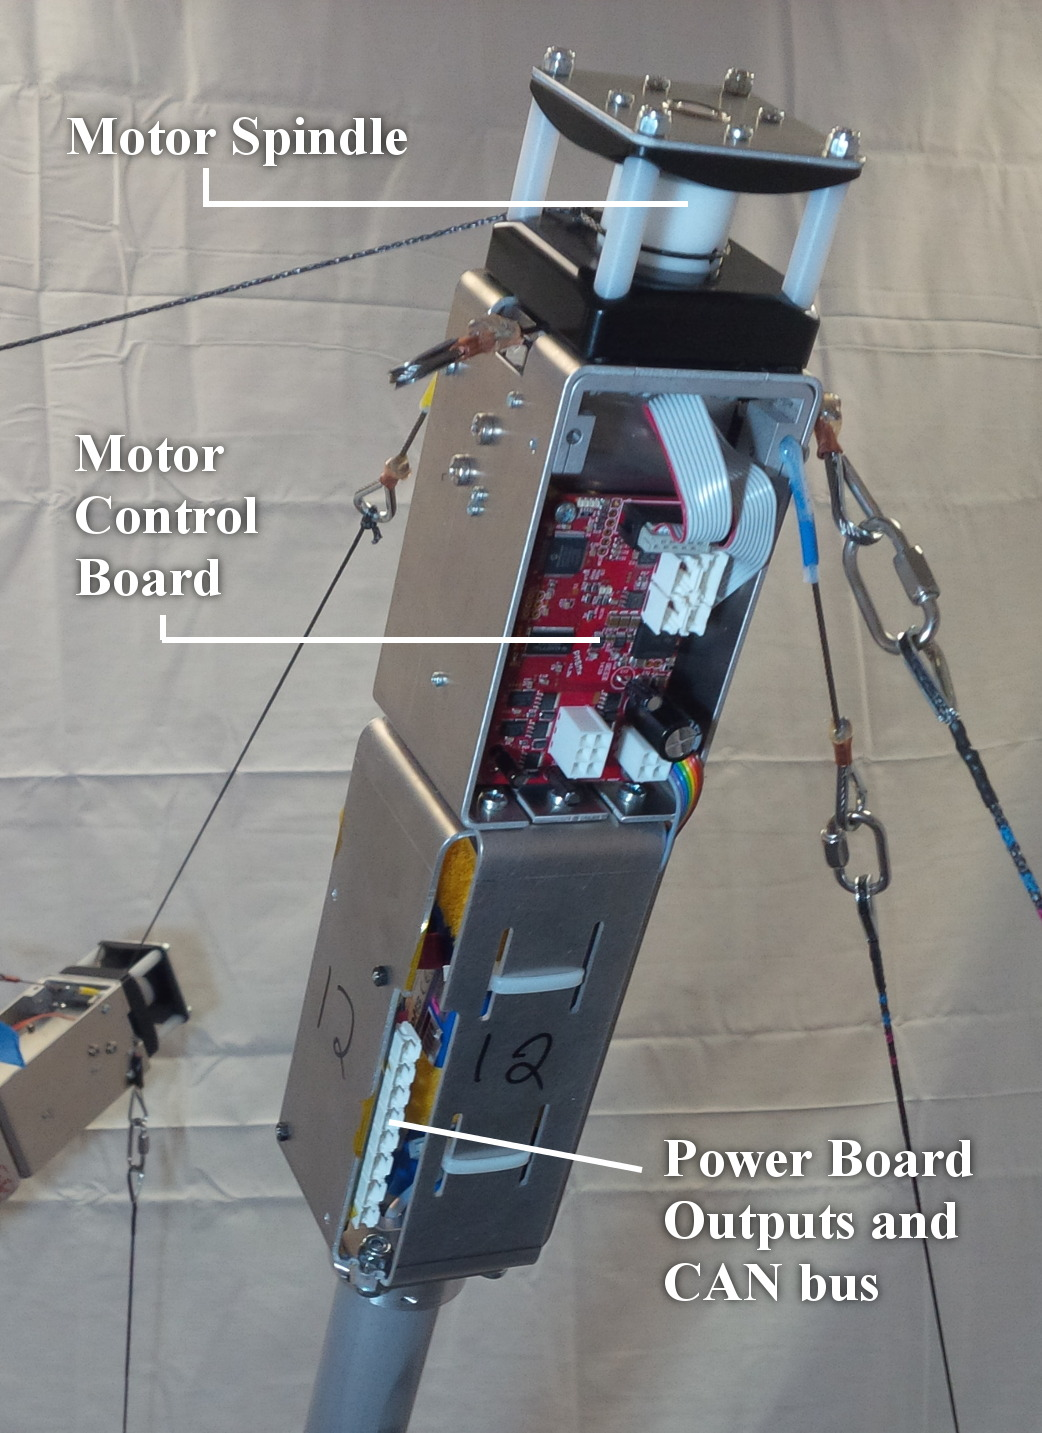
\includegraphics[width=0.5\columnwidth]{tex/img/endcap_upclose_motorboard_labelled_fixedfonts}
      \caption{MTR back side.}
      \label{fig:endcap_upclose_back}
\end{subfigure}
\caption{Fully assembled Modular Tensegrity Robot images on SUPERball}
\label{fig:fully_assembled_endcap}
\end{figure}

\section{Mechanical}
The main structural elements of the MTRs were kept simple to  enable  each  MTR  to  be self  contained  so  that  the  MTR  may be removed from the connecting rod as one whole unit.
The MTRs  are  held  onto  the  connecting  rods  by  a  simple tube  collar  for  easy  removal. 
There  are  5  sections  to MTR: a spring holder, battery holder, motor and electronics, cable actuation and routing, and a ground contact. 
Design parameters are shown in table \ref{design_req} in section \ref{modeling}.
The supporting metallic structural elements are made from 6061-T6 aluminum and machined plastic elements are Polyoxymethylene (commercially known as Delrin) unless otherwise noted.

\subsection{Spring Holder}
A  lesson  learned  from other tensegrity robots and the designer of ReCTeR~\cite{Caluwaerts2013rsif} was  that  externally  exposed springs are not ideal for a robotic system that would be interacting with a dynamic and unknown enviroment. 
The exposed springs get caught on objects and the assumption of near mass-less cables  can  no  longer  be  applied.  
On  the  MTR, an enclosed compression spring system was developed  to  alleviate  these  issues.  
Compression  springs were chosen so that during any unknown impact, the springs would not plastically deform. 
For \SB{}, a spring with a spring constant of \(998 Nm\) is attached to a passive cable element  and  a \(2850 Nm\) spring  is  attached  to  an  actuated cable.  
A  passive  spring was chosen with a total throw of \(23 cm\) to allow for pretension to be instated into the passive springs as well as to allow a wide dynamic compliant range.  
Since the actuated cables will be able to dynamically control pretension, a smaller throw spring was chosen to conserve space.
Figure \ref{fig:spring_holder} shows a closeup of how the spring holder functions.
How cables are attached to the springs inside the spring holder is explained in section \ref{routing}.

\begin{figure}[thpb]%{.5\textwidth}
      \centering
      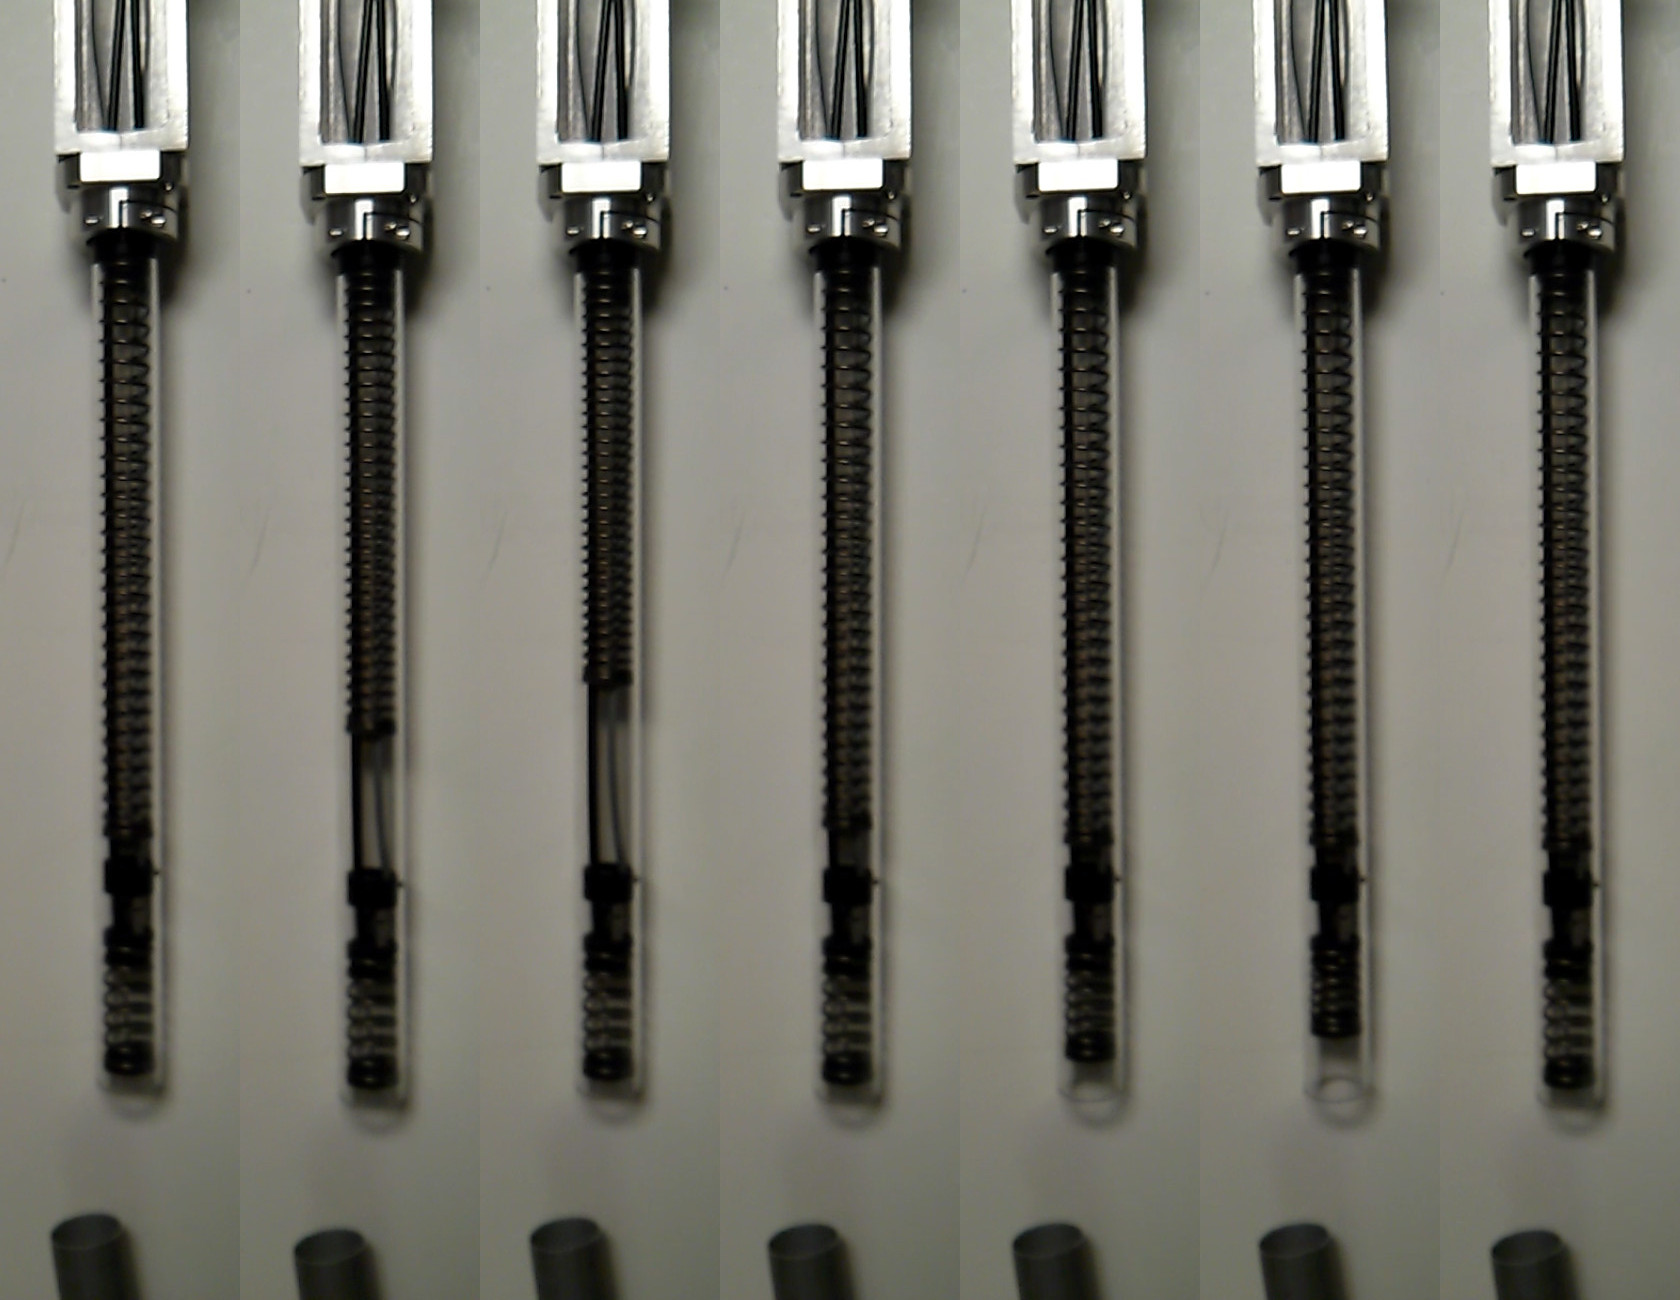
\includegraphics[width=0.8\columnwidth]{tex/img/double_spring_series}
      \caption{Time lapsed stills of spring compression in the MTR spring holder. Note that these stills are from a previous version of the MTR.}
      %\vspace{-0.5cm}
      \label{fig:spring_holder}
\end{figure}

\subsection{Battery Holder}
\label{battery_holder}
From the inception of \SB{}, enabling a self-contained power source which was easily accessible per MTR was a driving design parameter.
During the initial design and build of the \SB{}, it was known that the batteries where to be 24 volt lithium polymer but optimal size and shape of the battery was unknown due to a changing power profile.
Therefore, a battery holder with a simple securing mechanism which can handle a wide range of battery sizes was utilized.
Two hook and loop straps were used with simple slot cutouts to enable cinching around a generic lithium polymer battery.
The holder was also made large enough to hold the Power Board PCB board opposite of the battery.
As shown in section \ref{power_board}, the Power Board was designed to be an low profile to allow for a large battery within the holder.

\subsection{Motor and Electronics}
\label{mechanical:motor}
This section of the MTR used on \SB{} was mechanically designed around the Maxon EC-22 100 watt BLDC motor used for actuation. 
Each Maxon motor is \(22 mm\) in diameter and \(108 mm\) long with gearbox and encoder.
The output shaft is a \(6 mm\) diameter D shaft of length \(10.2 mm\).
A size requirement for how large the cross sectional diameter of the MTR could be was a limiting factor in designing the motor and electronic section.
The maximum diameter for any section used in the MTR was maximally limited to double the diameter of the connecting rod.
The idea for such a limitation was to keep the effective moment arm out from the center axis of any rod to a minimum.  
Due to the spring size and the need for a spring holder tube, the minimum diameter for the connecting rod was \(~35mm\) giving a maximum MTR diameter of \(70mm\).

The main component in the motor and electronic section of the MTR is the cable routing support bracket. 
This bracket plays three roles in the mechanical design: static support for the motor, support for the supporting material, and main exit support for the internal cable routing.
Figure \ref{fig:roller_guide} shows the cable routing support bracket above the pulley.
The actual motor mount was designed to be mechanically floating to enable torque sensing directly on the motor mount.
Thus, the cable routing support bracket sinks the reaction torque induced by the motor.
There are two electronic boards, the Sensor and Motor boards, which are mounted to brackets that straddle the motor.
Due to space limitations, these brackets are also load bearing components for the torsional forces induced by the motor.

\subsection{Cable Actuation and Routing}
\label{routing}
A simple spool design was implemented to directly actuate the cable. 
The spool directly couples to the motor shaft by sliding onto the D shaft.
A radial bearing supports the top of the spool and since the force vector applied to the spool by the actuated cable will never be just perpendicular to the spool, a thrust bearing was embedded into the bottom of the spool.
The thrust bearing sinks the trust force into the motor mount and each spool has the ability to slide along the the shaft's main axis. 
Since this thrust force is perpendicular to the torque of the motor, this force is not induced into the torque sensor built into the motor mount.

There are three other cables that connect to a MTR on \SB{}, though the device may support more with slight additions not explained here.
The cables used externally from the MTR are composed of Vectran braided cable and the cables used within the MTR are braided steel cabling. 
Two cables are routed through the MTR to the spring housing section and the other is terminated on the outside of the MTR.
Both routed cables enter the MTR through the cable routing support bracket mentioned in \ref{mechanical:motor}.
The cables are immediately routed around a rolling guide bearing to induce an approximate 90 degree bend to guide the cables towards the spring tube holder section, seen in figure \ref{fig:roller_guide}.
After the rolling guide bearing, the cables enter a PTFE tube to create a bowden cable to help route the cables around components within the MTR.
Once the cables reach their respective spring within the spring tube holder, the PTFE tube is terminated and the cable is routed through the spring and terminated using a copper compression sleeve.

\begin{figure}[thpb]
      \centering
      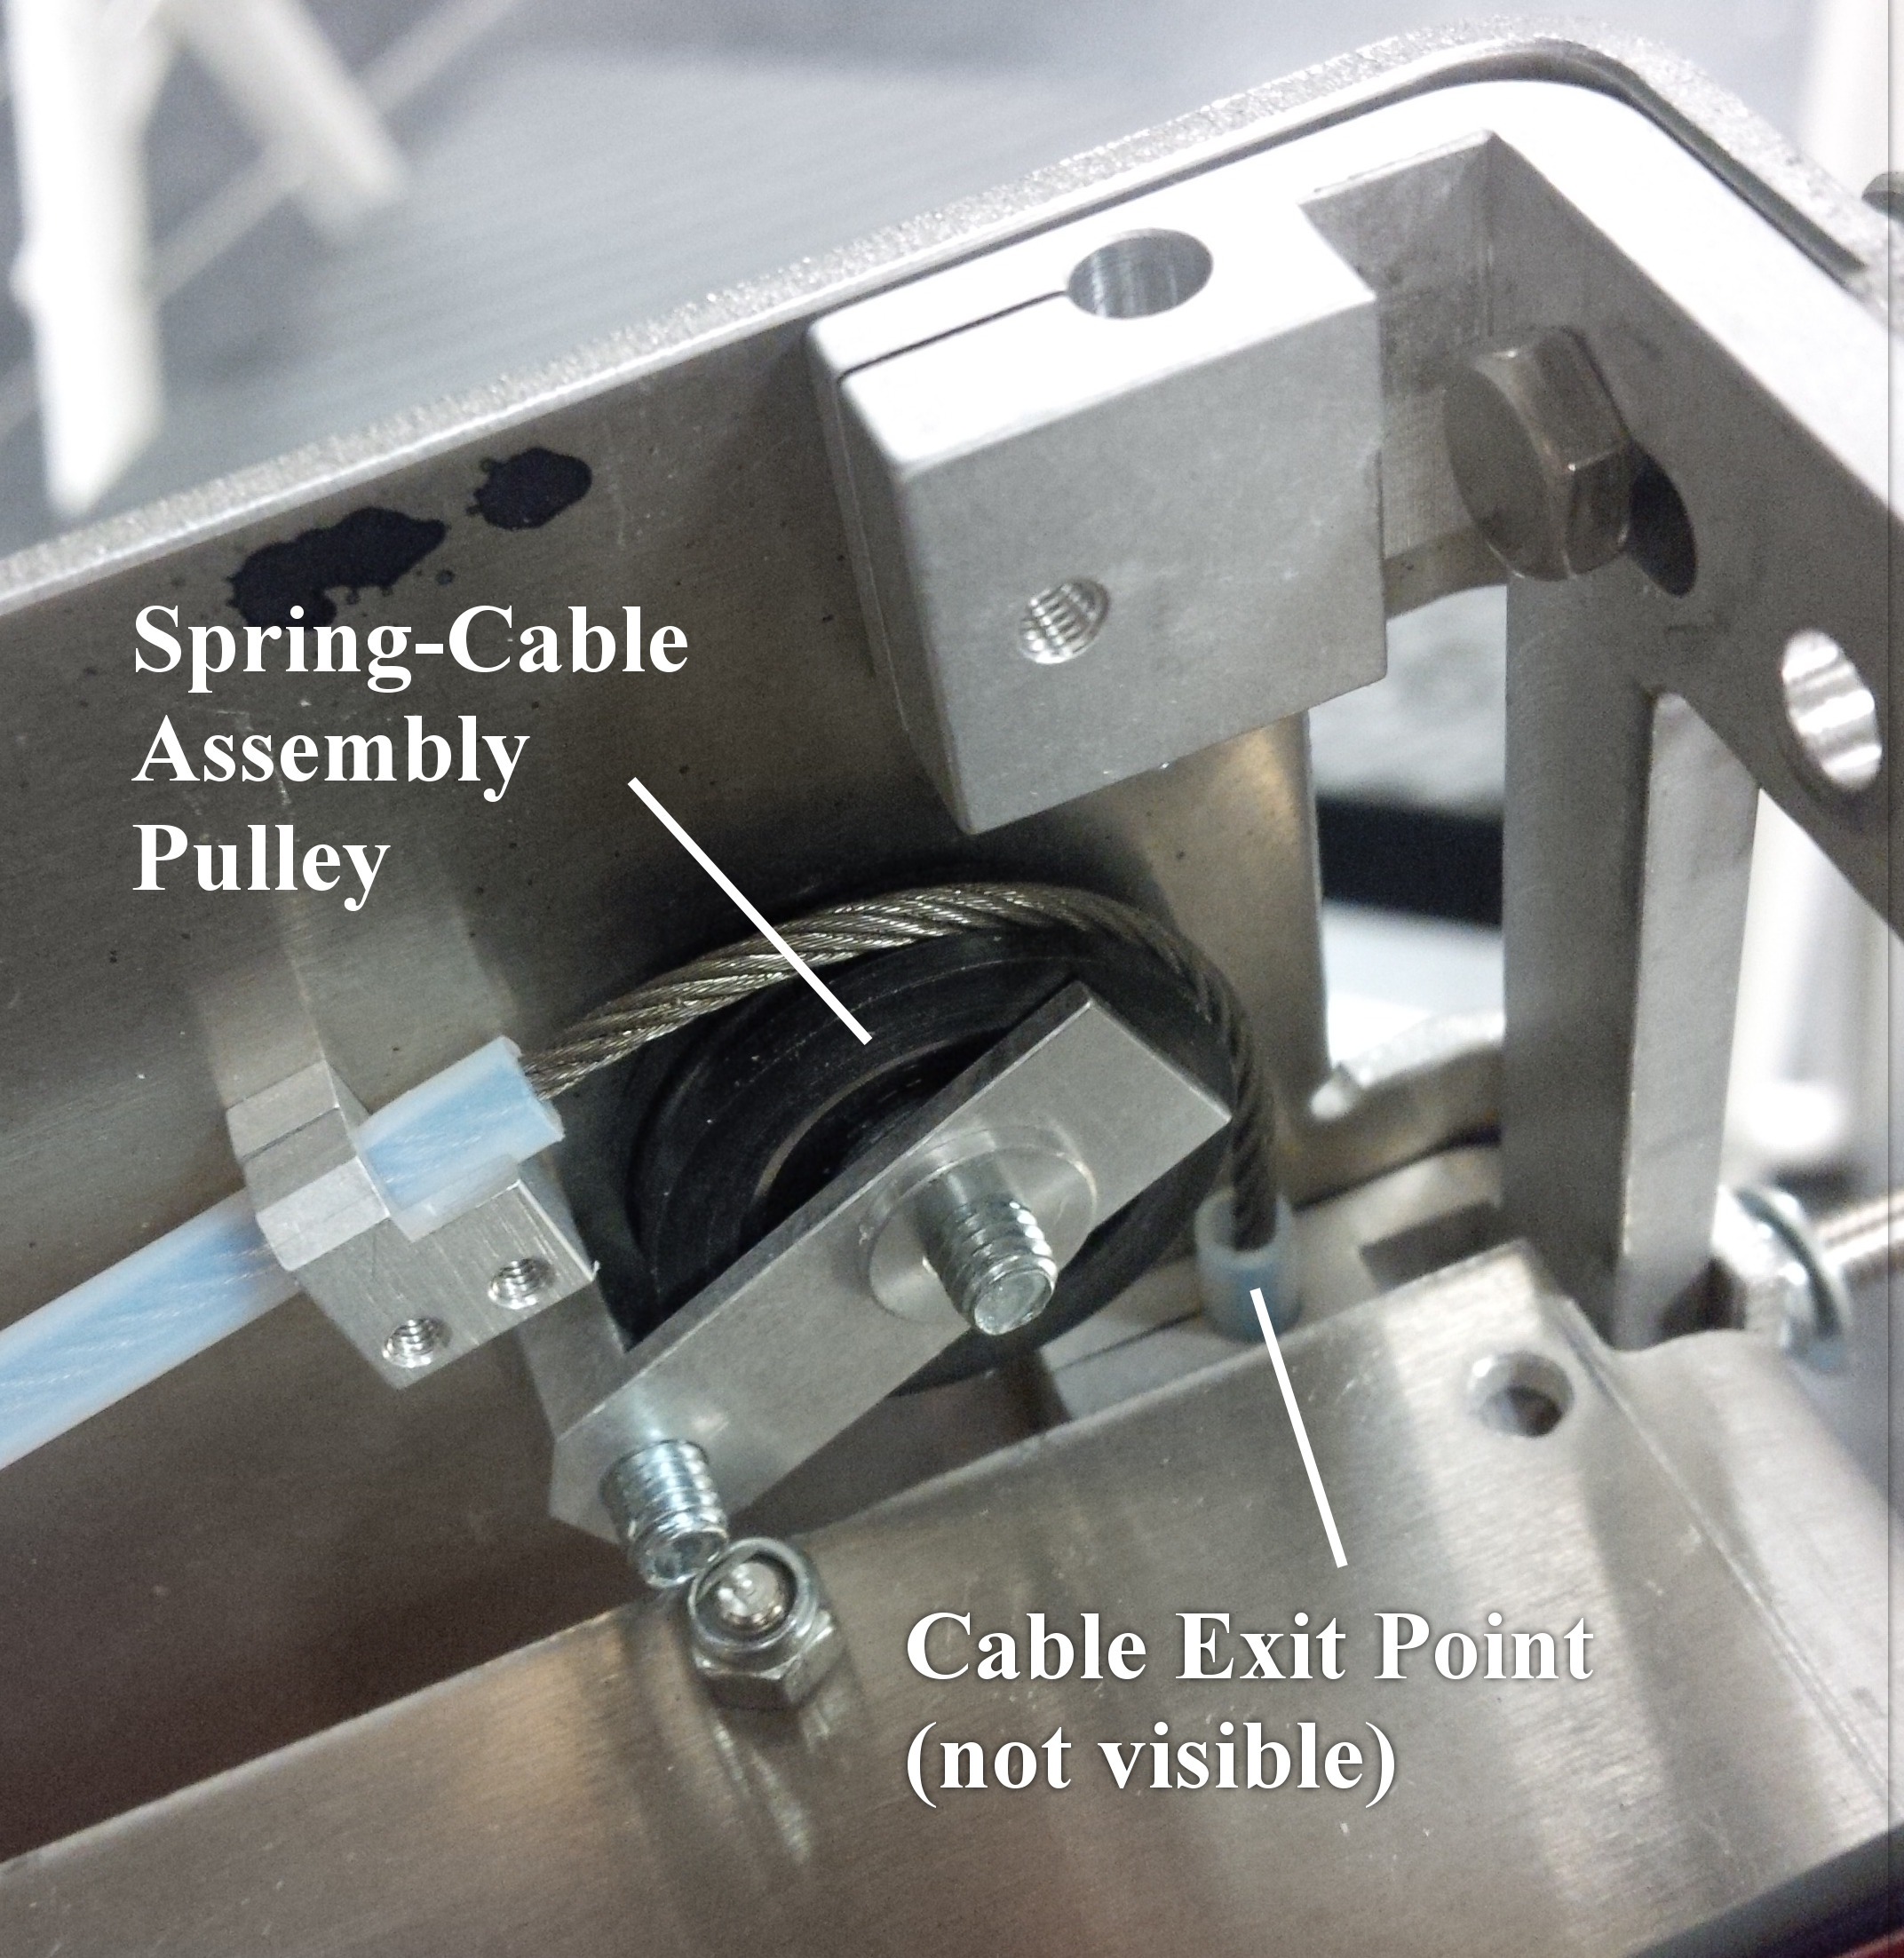
\includegraphics[width=0.6\columnwidth]{tex/img/cable_pulley_bearing_labelled_fixedfonts}
      \caption{Cable routing roller guide within an MTR.}
      \label{fig:roller_guide}
\end{figure}

\subsection{Ground Contact} 
This final section of the MTR is the simplest. 
To protect the MTR during locomotion, a 3D printed cap was manufactured to cover the end.
This part is designed with a diameter of \(80mm\) so that it is the only part of the MTR that contacts the ground during normal locomotion.
To decrease the impact shocks as the rod contacts a surface, compliant foam sheets are place between the 3D printed cap and the MTR.

\section{Electrical}
\SB{}'s electronics where developed with a focus on reliability, safety, and enabling distributed controls.
Another parameter was the ability to drive the 100W BLDC Maxon motors.
These main design criteria gave way to implement separate electronic boards based on their main function.
Each MTR has three custom Microchip dspic33e enabled PCB boards and the ability to house one ARM based computer called a Beagle Bone Black.
Each custom PCB is designed for very different purposes: A board to condition sensor data and run real-time control loops, a board to condition and distribute a 5.5V electronic power rail and a 24V motor power rail, and a board to control the 100W BLDC motor. 
The only requirements for each custom board is full CAN bus communication support and power conditioning for the 5.5V power rail.
The boards are simply named by their main purpose, thus Sensor, Power, and Motor respectively.
Though each MTR can house a Beagle Bone Black, \SB{} only has one per strut for cost saving and initial implementation simplicity. 

\subsection{Motor Board}
An initial driving parameter used during the design of SUPERball was the BLDC motor. 
During the design review for \SB{}, a lightweight motor with high power and efficiency was desired.
Thus, a Maxon brushless motor was a logical choice.
Table \ref{motor_parameters} shows the electrical properties of this motor.
In order to effectively drive this motor, a dedicated motor board was used on each MTR.
The main development of this board was engineered by Pavlo Manovi, and certain aspects of the board where tailored for our needs~\cite{Pavlo2014}.
The main components on the Motor board are the Microchip's 16-bit dsPIC33ep256mu506 micro-controller and the Texas Instruments DRV8303 three phase pre-driver.
Figure \ref{fig:motor_board} shows the current version of the motor board.

% \begin{table}[th]
% \centering
% \caption{100W Maxon BLDC Motor Parameters}
% \label{motor_parameters}
% \resizebox{\textwidth}{!}{%
% \begin{tabular}{|c|c|c|c|c|}
% \hline
% \multicolumn{5}{|c|}{Motor without Gearbox} \\ \hline
% \begin{tabular}[c]{@{}c@{}}Nominal Voltage\\  (V)\end{tabular} & \begin{tabular}[c]{@{}c@{}}No Load Speed \\ (rpm)\end{tabular} & \begin{tabular}[c]{@{}c@{}}No Load Current \\ (mA)\end{tabular} & \begin{tabular}[c]{@{}c@{}}Stall Torque \\ (mNm)\end{tabular} & \begin{tabular}[c]{@{}c@{}}Max Efficiency \\ (\%)\end{tabular} \\ \hline
% 24 & 26,500 & 16.8 & 691 & 92 \\ \hline
% \end{tabular}
% }
% %\centering
% %\resizebox{\textwidth}{!}{%
% \begin{tabular}{|c|c|c|c|c|}
% \hline
% \multicolumn{5}{|c|}{Gearbox} \\ \hline
% Reduction & Number of Stages & \begin{tabular}[c]{@{}c@{}}Max Continuous \\ Torque (Nm)\end{tabular} & \begin{tabular}[c]{@{}c@{}}Max Peak Torque \\ (Nm)\end{tabular} & Max Efficiency (\%) \\ \hline
% 109:1 & 3 & 3 & 3.5 & 59 \\ \hline
% \end{tabular}
% %}
% \end{table}

% Please add the following required packages to your document preamble:
% \usepackage[table,xcdraw]{xcolor}
% If you use beamer only pass "xcolor=table" option, i.e. \documentclass[xcolor=table]{beamer}
\begin{table*}[th]
\centering
\caption{100W Maxon BLDC Motor Parameters}
\label{motor_parameters}
\begin{center}%
\resizebox{\columnwidth}{!}{%
\begin{tabular}{|ccccc|}
\hline
\multicolumn{5}{|c|}{Motor without Gearbox}                                                                                                                         \\ \hline
Nominal Voltage (V) & \cellcolor[HTML]{C0C0C0}No Load Speed (rpm) & No Load Current (mA)       & \cellcolor[HTML]{C0C0C0}Stall Torque         & Max Efficiency (\%) \\
24                  & \cellcolor[HTML]{C0C0C0}26,500              & 16.8                       & \cellcolor[HTML]{C0C0C0}691                  & 92                  \\ \hline
\multicolumn{5}{|c|}{Gearbox}                                                                                                                                       \\ \hline
Reduction           & \cellcolor[HTML]{C0C0C0}Number of Stages    & Max Continuous Torque (Nm) & \cellcolor[HTML]{C0C0C0}Max Peak Torque (Nm) & Max Efficiency (\%) \\
109:1               & \cellcolor[HTML]{C0C0C0}3                   & 3                          & \cellcolor[HTML]{C0C0C0}3.5                  & 59                  \\ \hline
\end{tabular}
}
\end{center}
\end{table*}

\subsection{Sensor Board and Beagle Bone Black}
\label{sensor_bbb}
The sensor board was originally designed as the main processing unit on a MTR. 
However, the design and building process has lead to the coupling of the sensor board with a Beagle Bone Black.
For a detailed explanation of why the Beagle Bone Black was integrated into the system, please refer to \ref{communication}.

The current version of the sensor board was developed as a daughter board for the Beagle Bone Black.
The board mates to the Beagle Bone Black through two double row 46 pin headers and provides power and CAN communication to the ARM board.
The main processing unit on the sensor board is Microchip's 16-bit dsPIC33ep128gp506 micro-controller.
Environmental sensing is enabled by a 9DOF inertial measurement unit (IMU) and a 24-bit analog to digital converter (ADC) configured in a half wheat-stone bridge configuration.
The IMU is comprised of Invensense's MPU6000 mastered to Freescale's MAG3110 magnetometer, and the ADC is Analog Device's AD7193.

The Beagle Bone Black is a open-source hardware single-board computer inspired by the BealgBoard, the larger predecessor developed by Texas Instruments as an educational tool.
The main processor on the board is a Sitara ARM Cortex-A8 processor running at 1Ghz and capable of running a full ARM based operating system (OS).
The processor is also able to interface directly with low level communication protocols such as CAN, UART, SPI, and I2C.
To meet our memory and speed requirements, a custom kernel was built with only the modules needed by our system.
On top of this kernel, the Beagle Bone Black is running a ROS (Robot Operating System, see section \ref{communication} for more detials) enabled Ubuntu ARM 14.04.1 LTS OS.

A new feature developed is the integration of DecaWave's DWM1000 module for relative distance measurements.
Legacy components no longer utilized on the sensor board for mounting an XBee device are being used with a custom DWM1000 breakout board.
The small breakout was designed to integrate the DWM1000 module into where the XBee device was originally mounted.
Figure \ref{fig:sensor_board} shows a prototype of the sensor board mounted to a Beagle Bone Black.

\subsection{Power Board}
\label{power_board}
The power board was design to enable safety, both for a person working near \SB{} and for the electronics, as well as conditioning input power to both a 5.5V and a 24V rail.
The board was also designed with a minimal height profile allowing for larger batteries to be placed near the board.
See section \ref{battery_holder}, to view the section which houses the power board.
The main idea of safety is focused around operating the 100W BLDC motors, thus a two battery system was implemented.
A small battery is used for starting the micro-controller boards but not capable of producing 24V needed by the motor, and a large battery is used during main operation of the MTR.
The two batteries are a 160 milli-amp-hour 1-cell and a 3 amp-hour 6-cell lithium polymer batteries, named the back-up and the main receptively.

To enable the 24V power, multiple input conditions should be met and fed into an analog and-gate equivalent circuit.
The input conditions are: a physical switch located on the MTR, a digital logic pin from the power board's micro-controller, power being applied by the back-up battery, and a signal coming from a dedicated 8-bit micro-controller monitoring a pulsed wireless 2.4Ghz signal.
If any one of these conditions go false, the entire 24V rail is disabled.
There are also fuses on both the 24V and 5.5V line to protect all the micro-controller circuits from shorts.
Figure \ref{fig:connection_diagram} shows a basic connection diagram for the power lines.

The main processing unit on the power board is Microchip's 16-bit dspicPIC33ep128mc506 mirco-controller.
The wireless "kill switch" monitoring mirco-controller is Mircochip's 8-bit PIC12(L)F1571/2 mirco-controller.
This chip monitors a known pulse width being communicated by a Nordic Semiconductor nRF24L01 breakout board with antenna.
The pulsed signal is sent by a hand held unit off the robot.
When a shut off command is sent or the PIC12's watchdog timer is triggered from a loss in wireless signal, the logic signal sent from the PIC12 is turned to false disabling the 24V power rail. 
5.5V power is either supplied by the back-up battery or the main battery using a custom boost or buck switching circuit, receptively.
The 24V rail is supplied directly from the main 6-cell battery when all input logic is enabled.
Figure \ref{fig:power_board} shows the power board. 

\begin{figure}[thpb]
\begin{subfigure}{.3\textwidth}
      \centering
      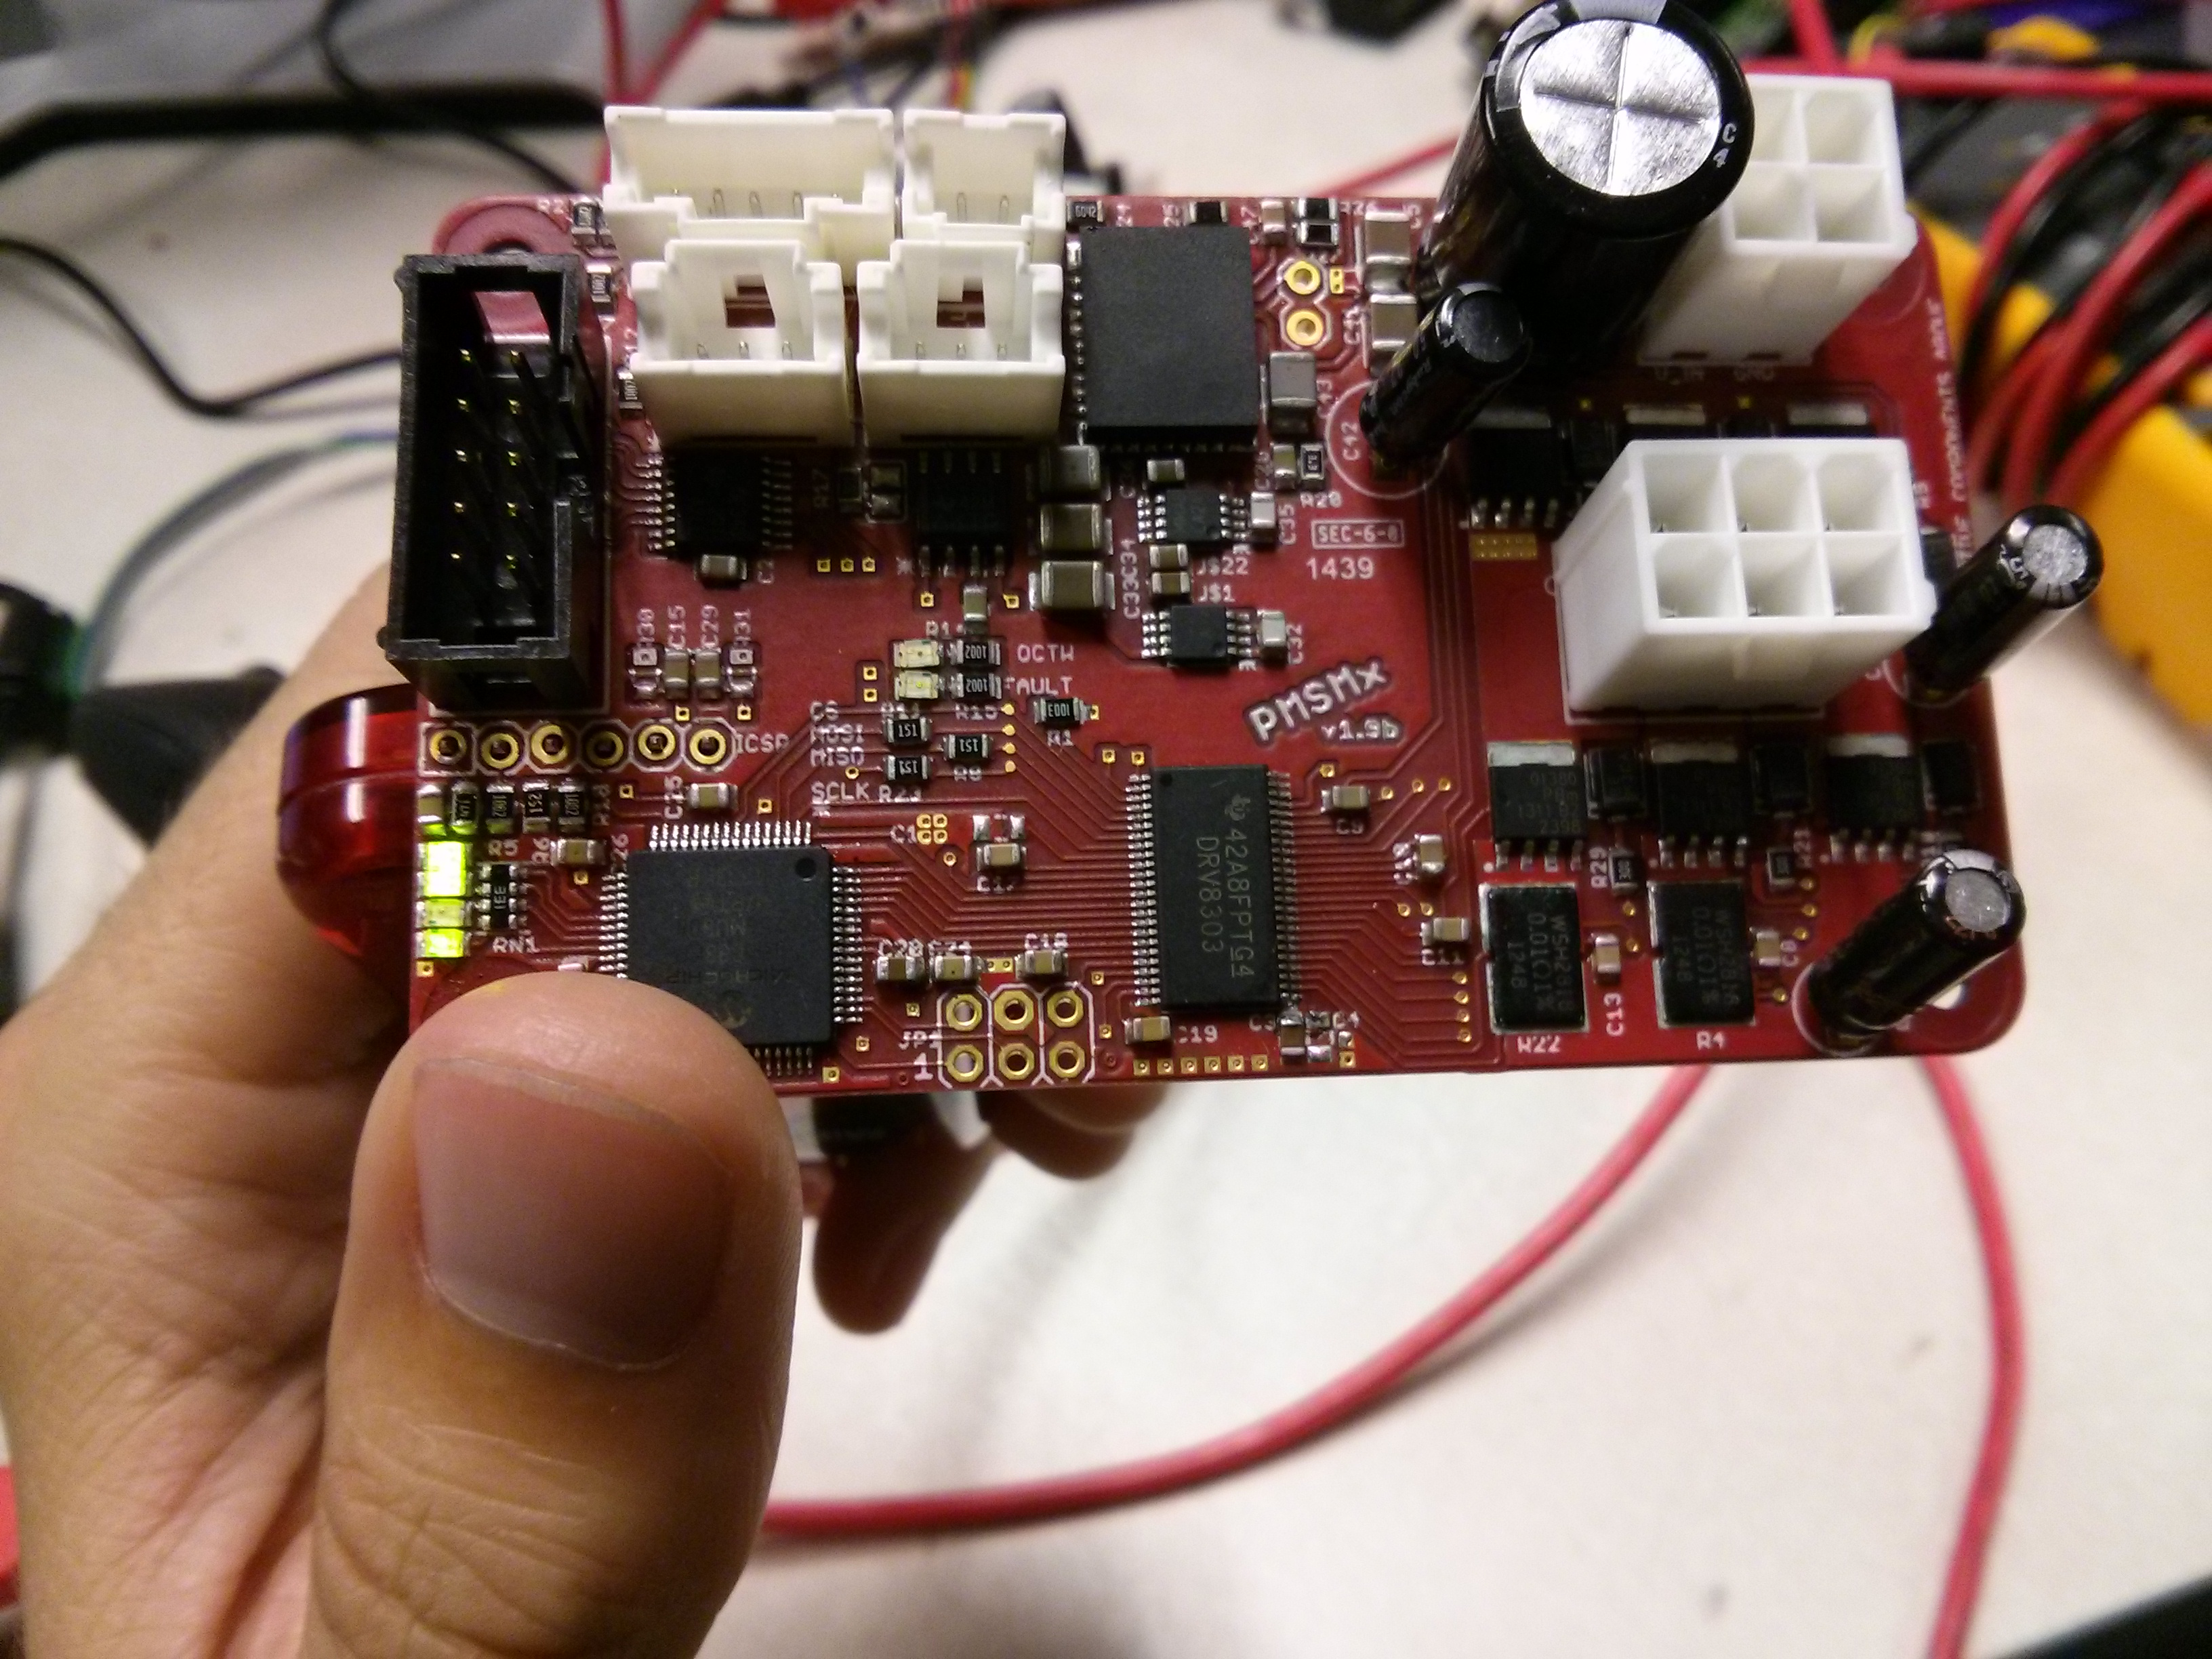
\includegraphics[width=\columnwidth]{tex/img/motor_board}
      \caption{Motor Board}
      \label{fig:motor_board}
\end{subfigure}
\begin{subfigure}{.3\textwidth}
      \centering
      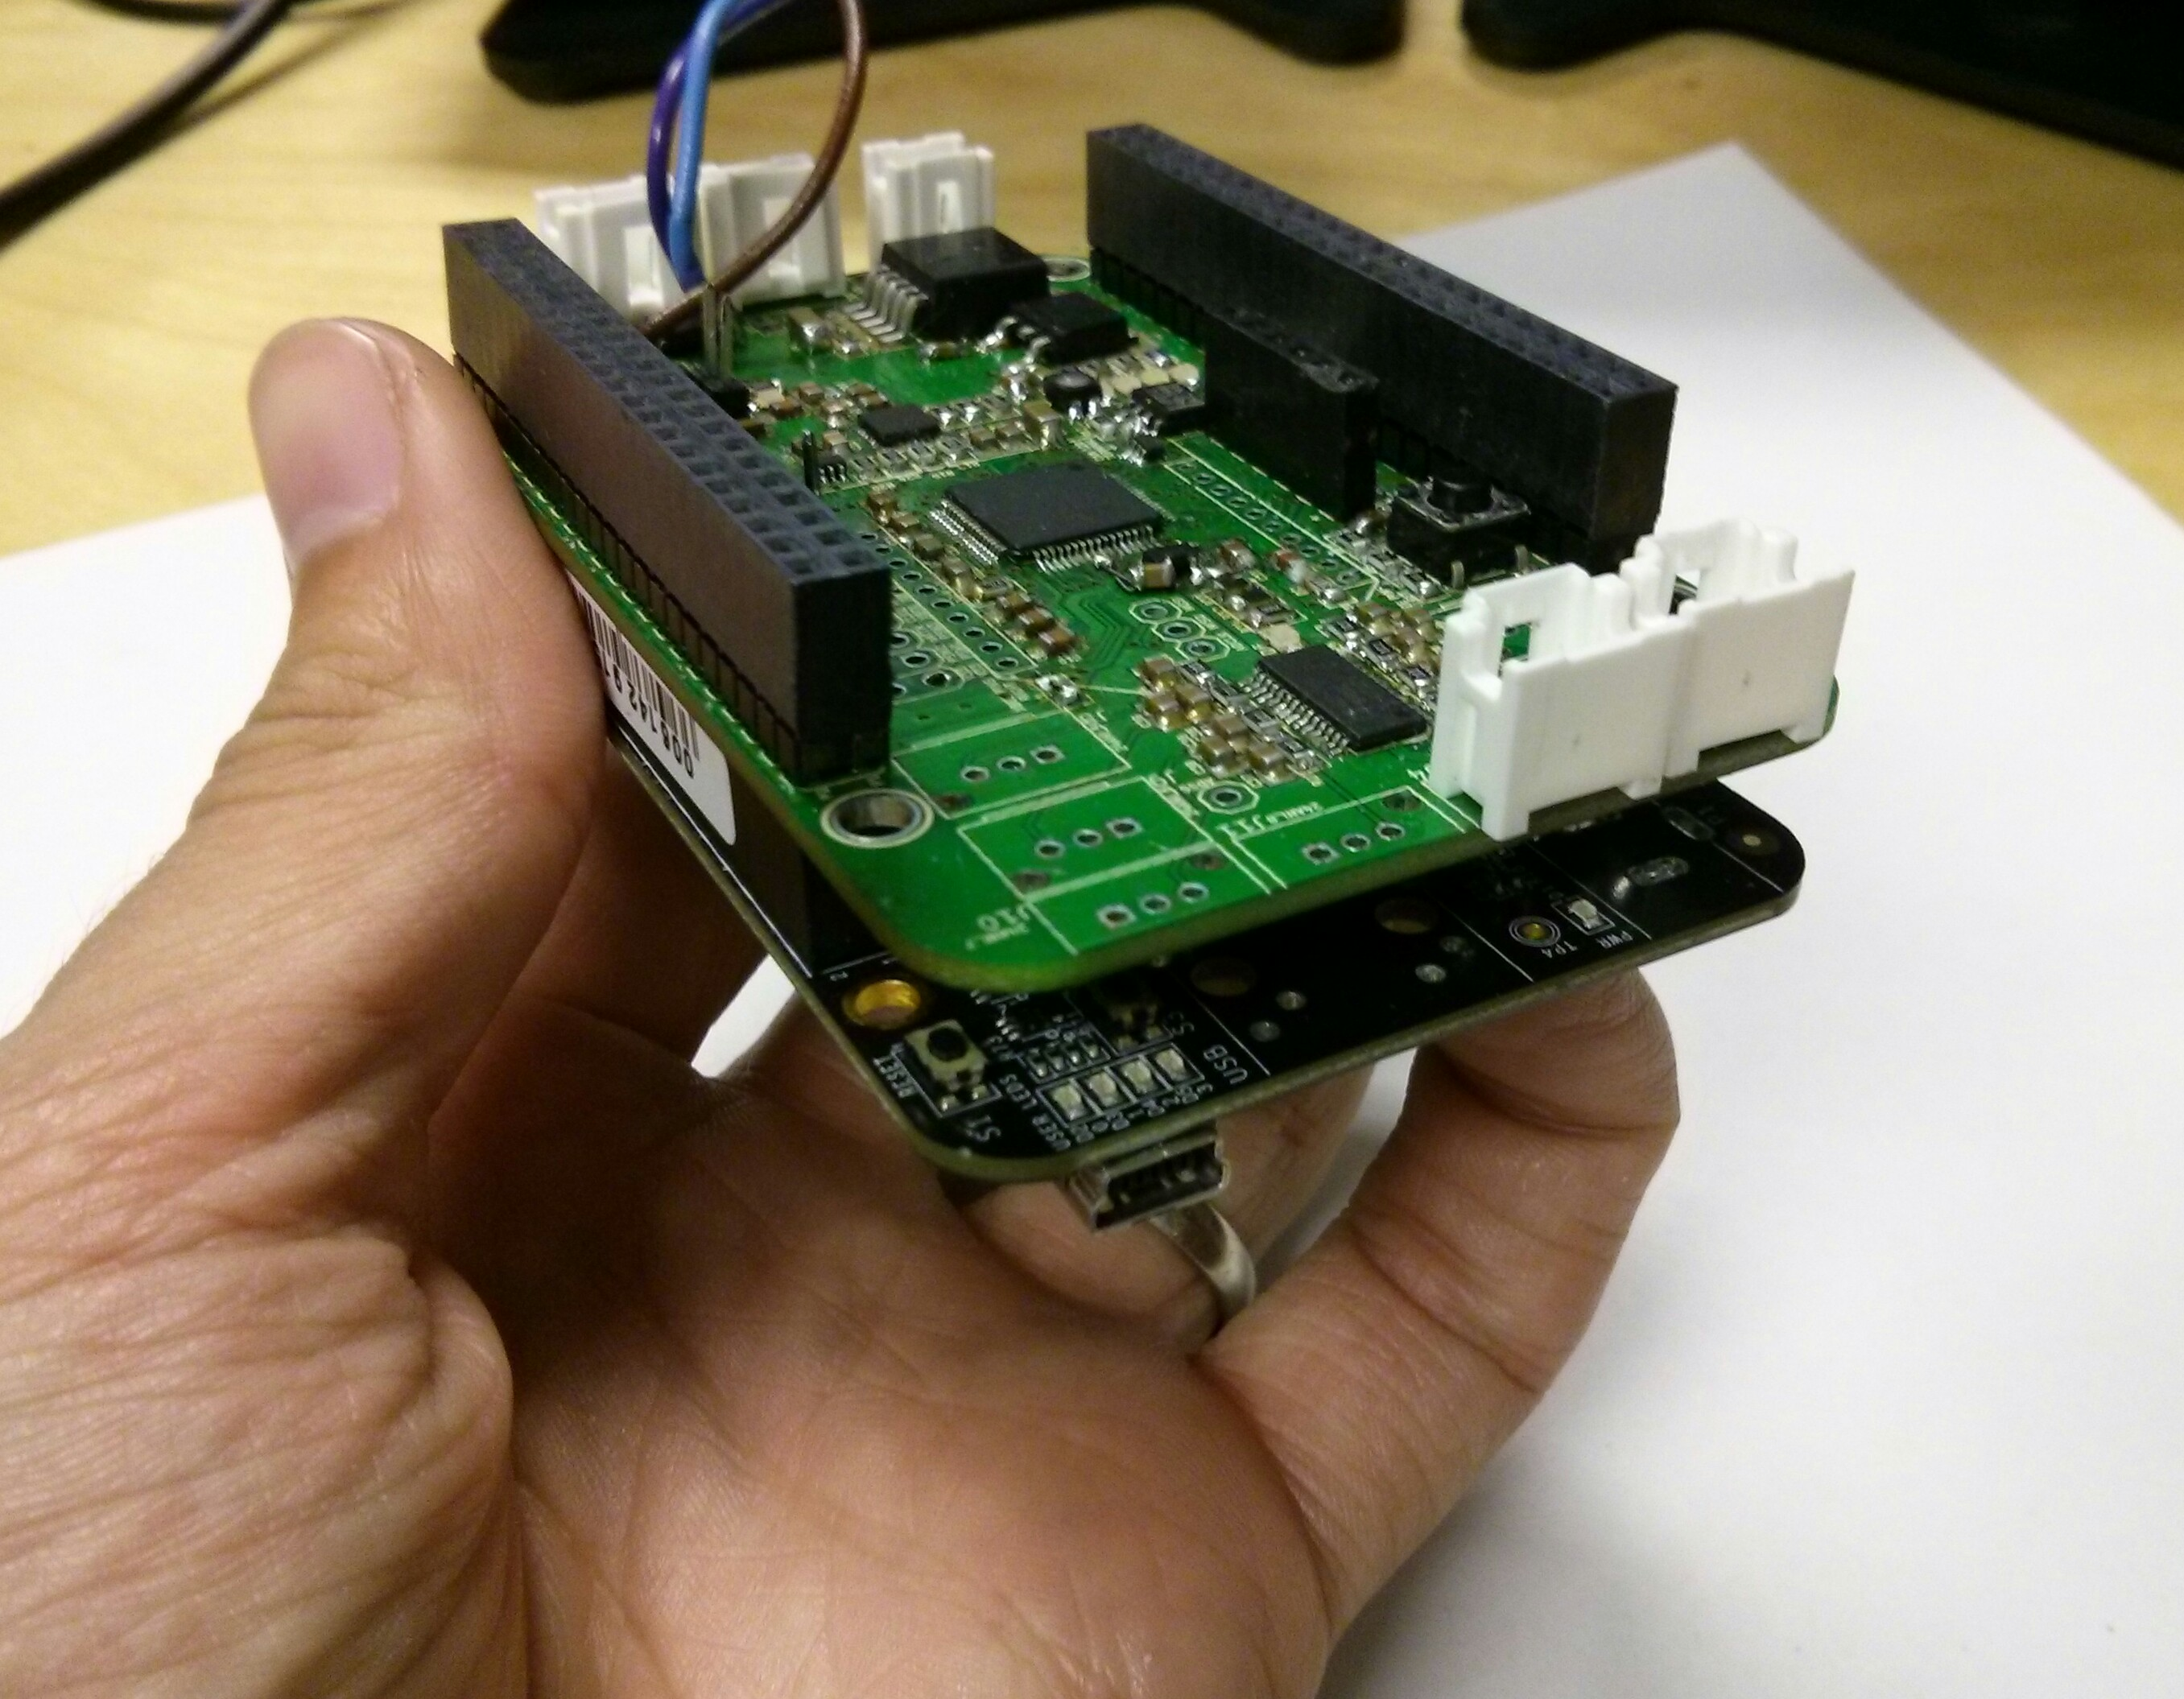
\includegraphics[width=\columnwidth]{tex/img/sensor_board}
      \caption{Early Prototype of the \\Sensor Board}
      \label{fig:sensor_board}
\end{subfigure}
\begin{subfigure}{.3\textwidth}
      \centering
      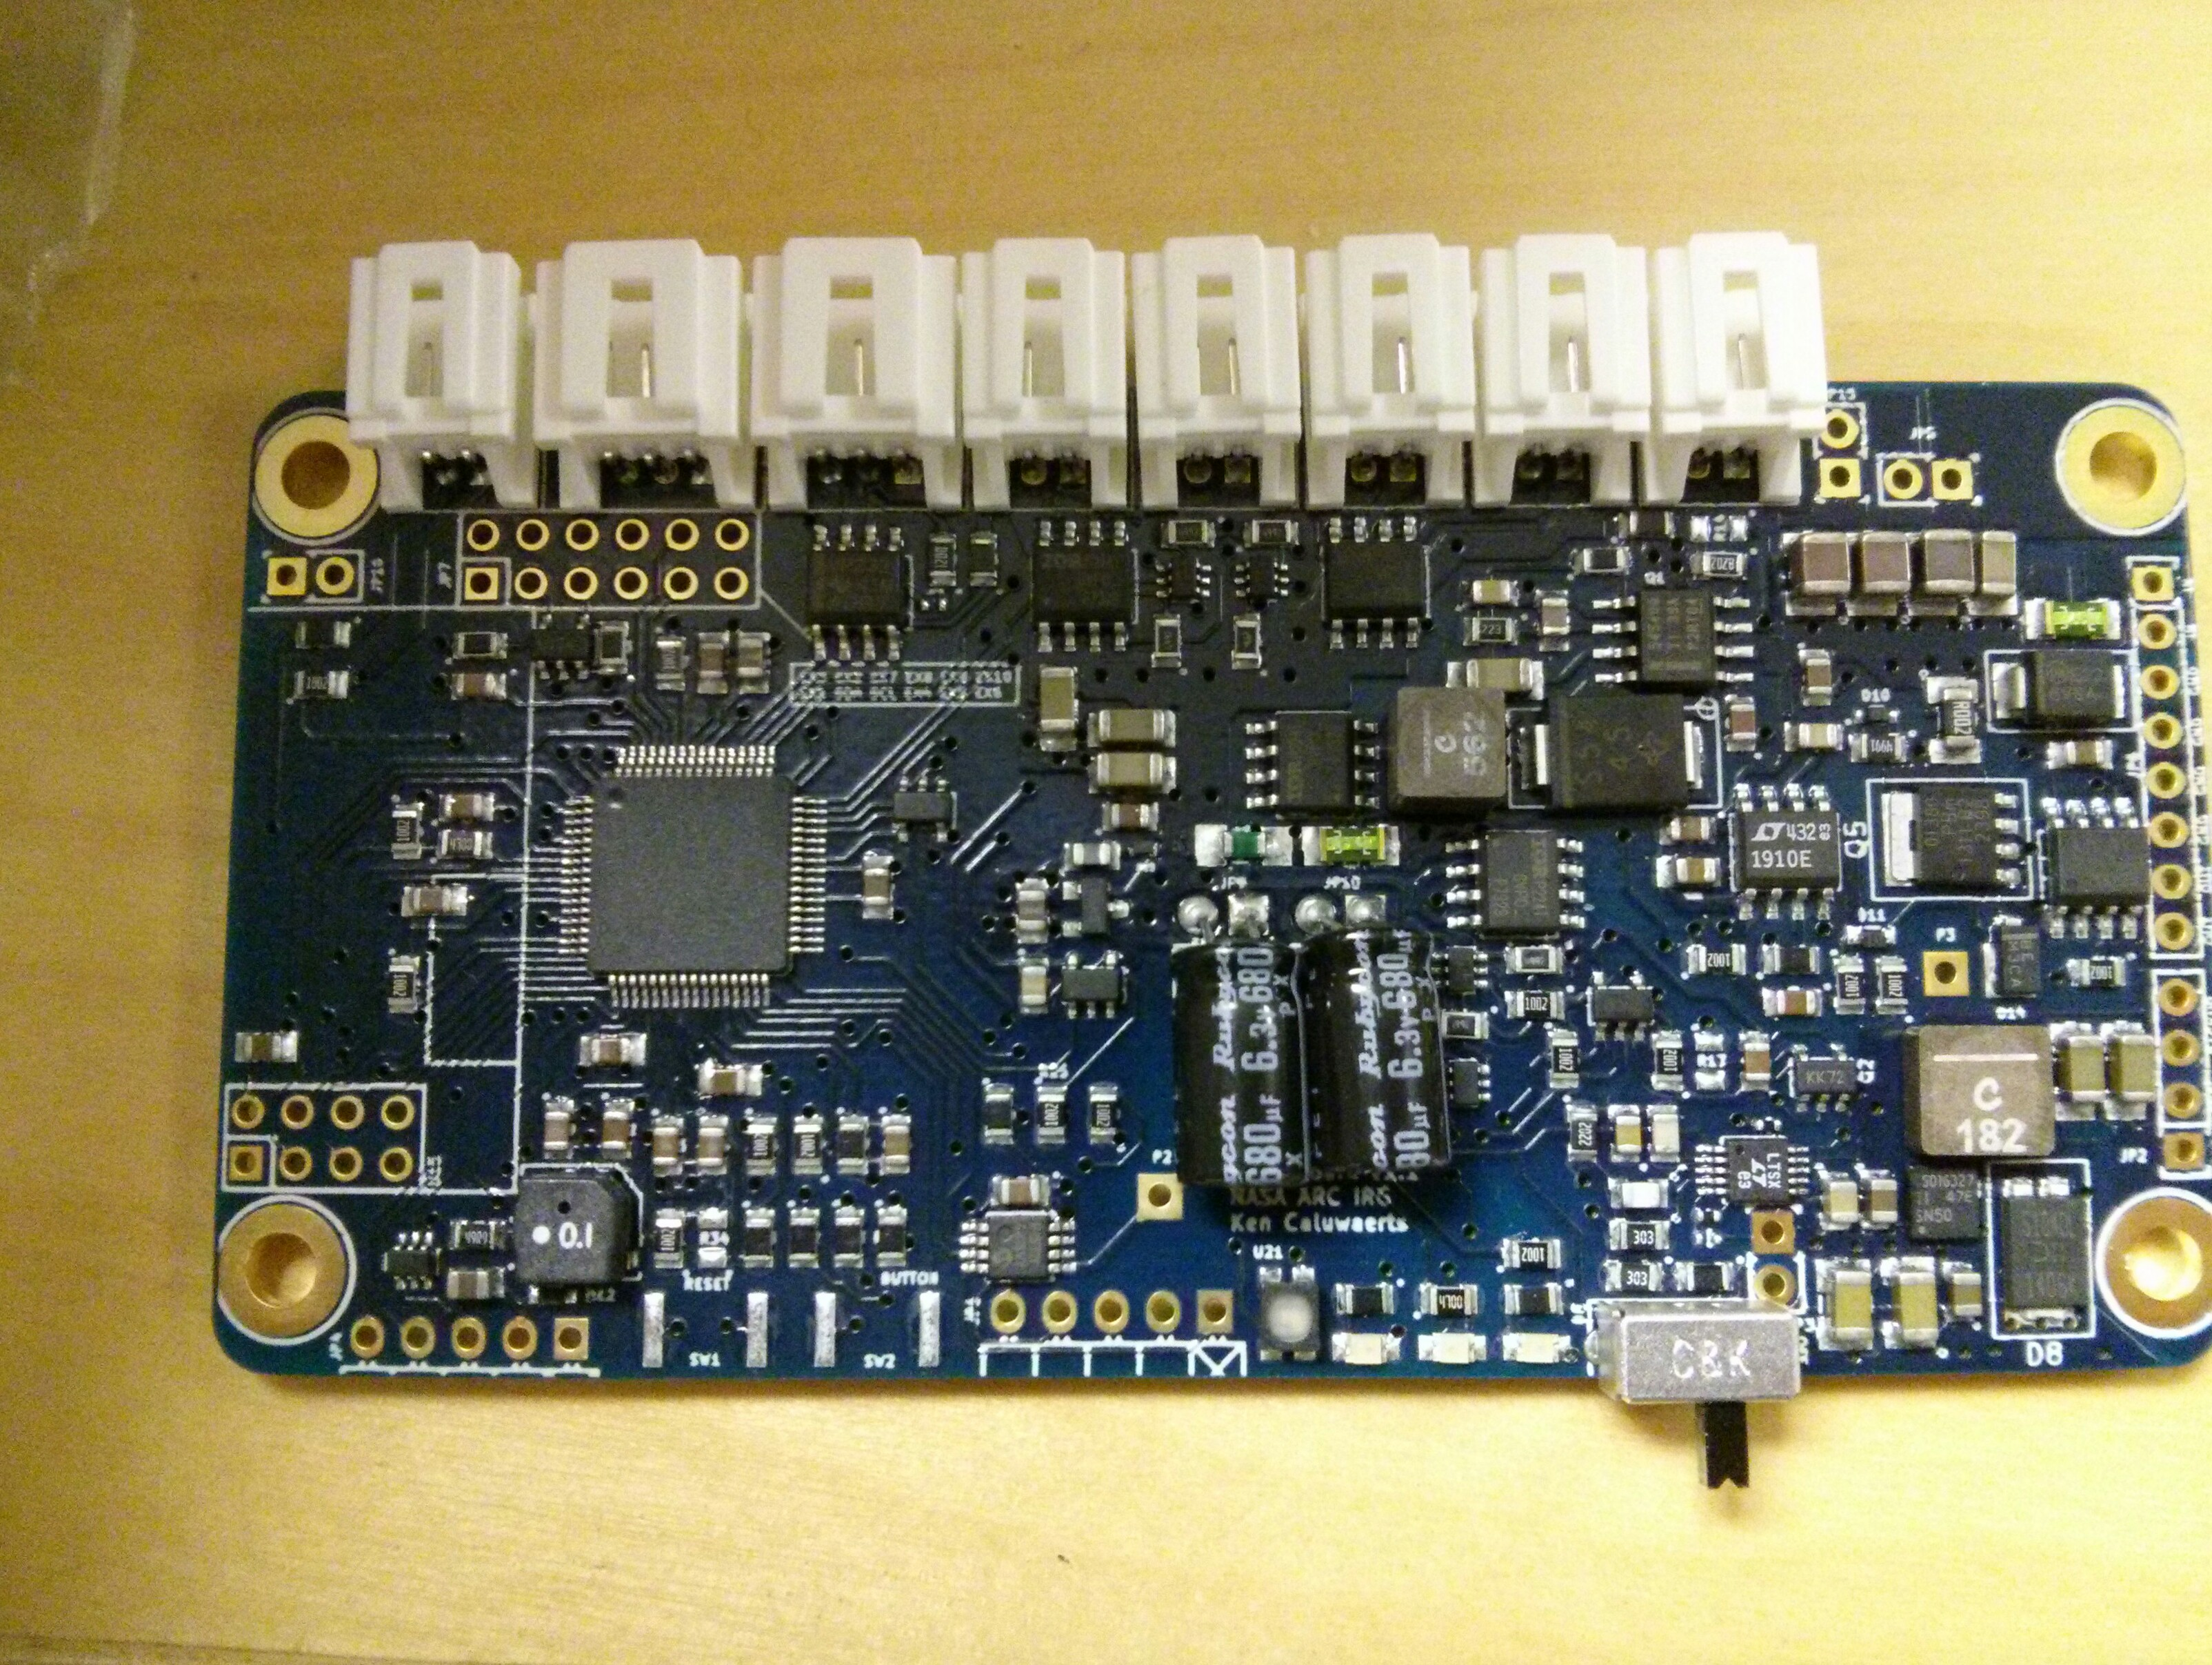
\includegraphics[width=\columnwidth]{tex/img/power_board}
      \caption{Power Board without nRF24l01 wireless chip}
      \label{fig:power_board}
\end{subfigure}
\caption{Pictures of each of the main micro-controller boards on an MTR.}
\label{fig:MTR_uC_boards}
\end{figure}

\section{Communication}
\label{communication}

Communication on \SB{} was designed around a desire to have each rod of the tensegrity system unteathered from any other part of the system.
Two wireless protocols as well as a wired Controller Area Network, or CAN, bus were implemented.
The two main wireless protocols are WiFi for main data communication and a 2.4GHz channel for wireless enabling/disabling of motor power for safety.
Figure \ref{fig:connection_diagram} shows how power and communication are connected for a single MTR and figure \ref{fig:ros_diagram} shows the connections for \SB{}'s wireless communications.

\begin{figure}[thpb]%{.5\textwidth}
      \centering
      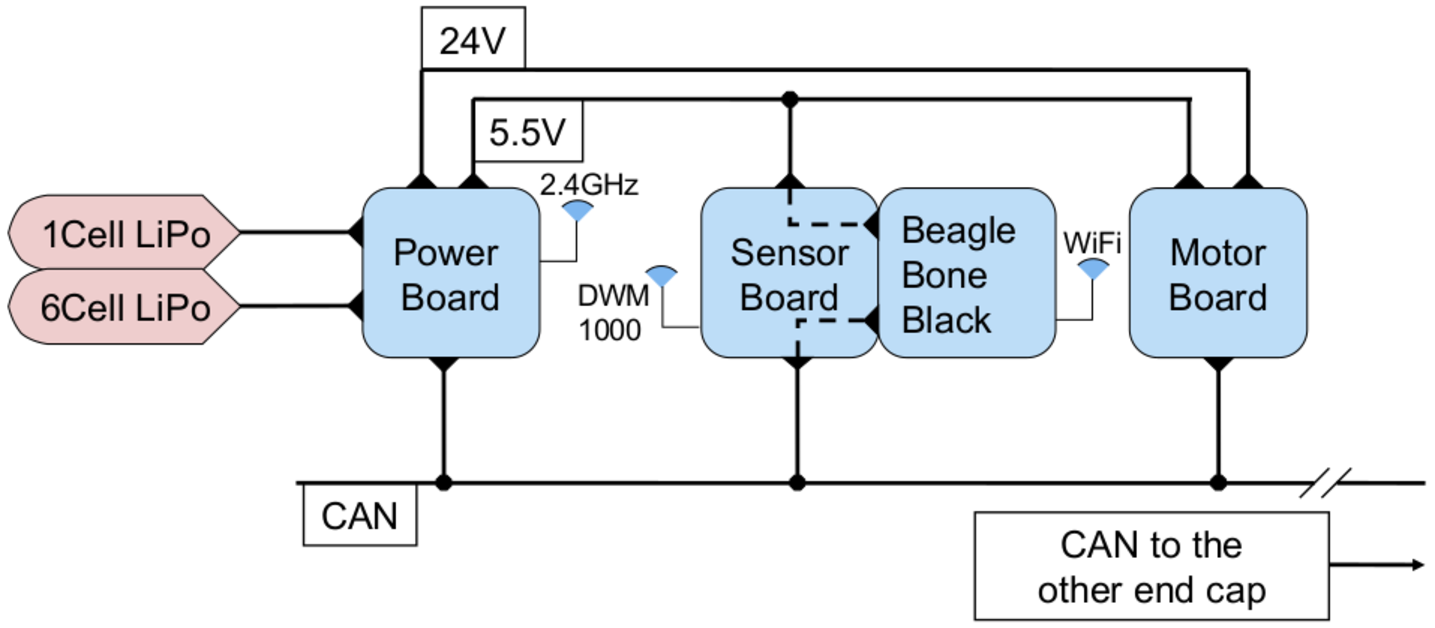
\includegraphics[width=0.8\columnwidth]{tex/img/hard_wire_connection}
      \caption{This is a connection diagram for power and communication for a MTR on \SB{}.}
      %\vspace{-0.5cm}
      \label{fig:connection_diagram}
\end{figure}

\subsection{CAN Bus}
A communication design was desired that would be robust, extensible, and work over long distances.
A CAN bus fits these main requirements and was implemented to be the main communication between all controllers on a single rod.
Since the CAN bus is a physical layer standard, a communication protocol is usually required to get a robust and extensible network.
A widely accepted protocol that has been well tested and understood, is the CANOpen protocol \cite{boterenbrood2000canopen}.
CANOpen defines the addressing scheme, several small communication protocols and an application layer defined by a device profile.
Some of the smaller communication protocols supported by CANOpen are device monitoring and communication between nodes, network management, and a simple transport layer for message processing.
This open source protocol is freely distributed and has many open and closed source implementations.
The CANOpen implementation used for \SB{} is the CANFestival project which focuses on implementing the basic protocol while maintaining a small code base and low computational load for embedded systems.
Each mirco-controller and Bealge Bone Black are able to run the entire CANFestival project code in less than \(150 \mu s\) under worst case scenarios.
The physical layer CAN bus is running at \(1 Mbit/s\) 

\subsection{WiFi and the Robot Operating System}
The Robot Operating System, or ROS, is a collection of software to provide operating system functionality on a network linked computer cluster. 
Message-passing and packet management works agnostic to the network layer, allowing information to be passed from one ROS enabled node to any other ROS enabled node on a network.
Figure \ref{fig:ros_diagram} shows a basic representation of how this message-passing works on the \SB{} ROS network.

As explained in section \ref{sensor_bbb}, enabling each rod is a ROS node was the driving reason to have at least one ARM based chip on every rod.
Since the Beagle Bone Black is also on the CAN bus, it's main function is to sniff the CAN network and send new information out to the ROS network.
This enables for near real time data analysis and for time stamped data logging on \SB{}.

\begin{figure}[thpb]%{.5\textwidth}
      \centering
      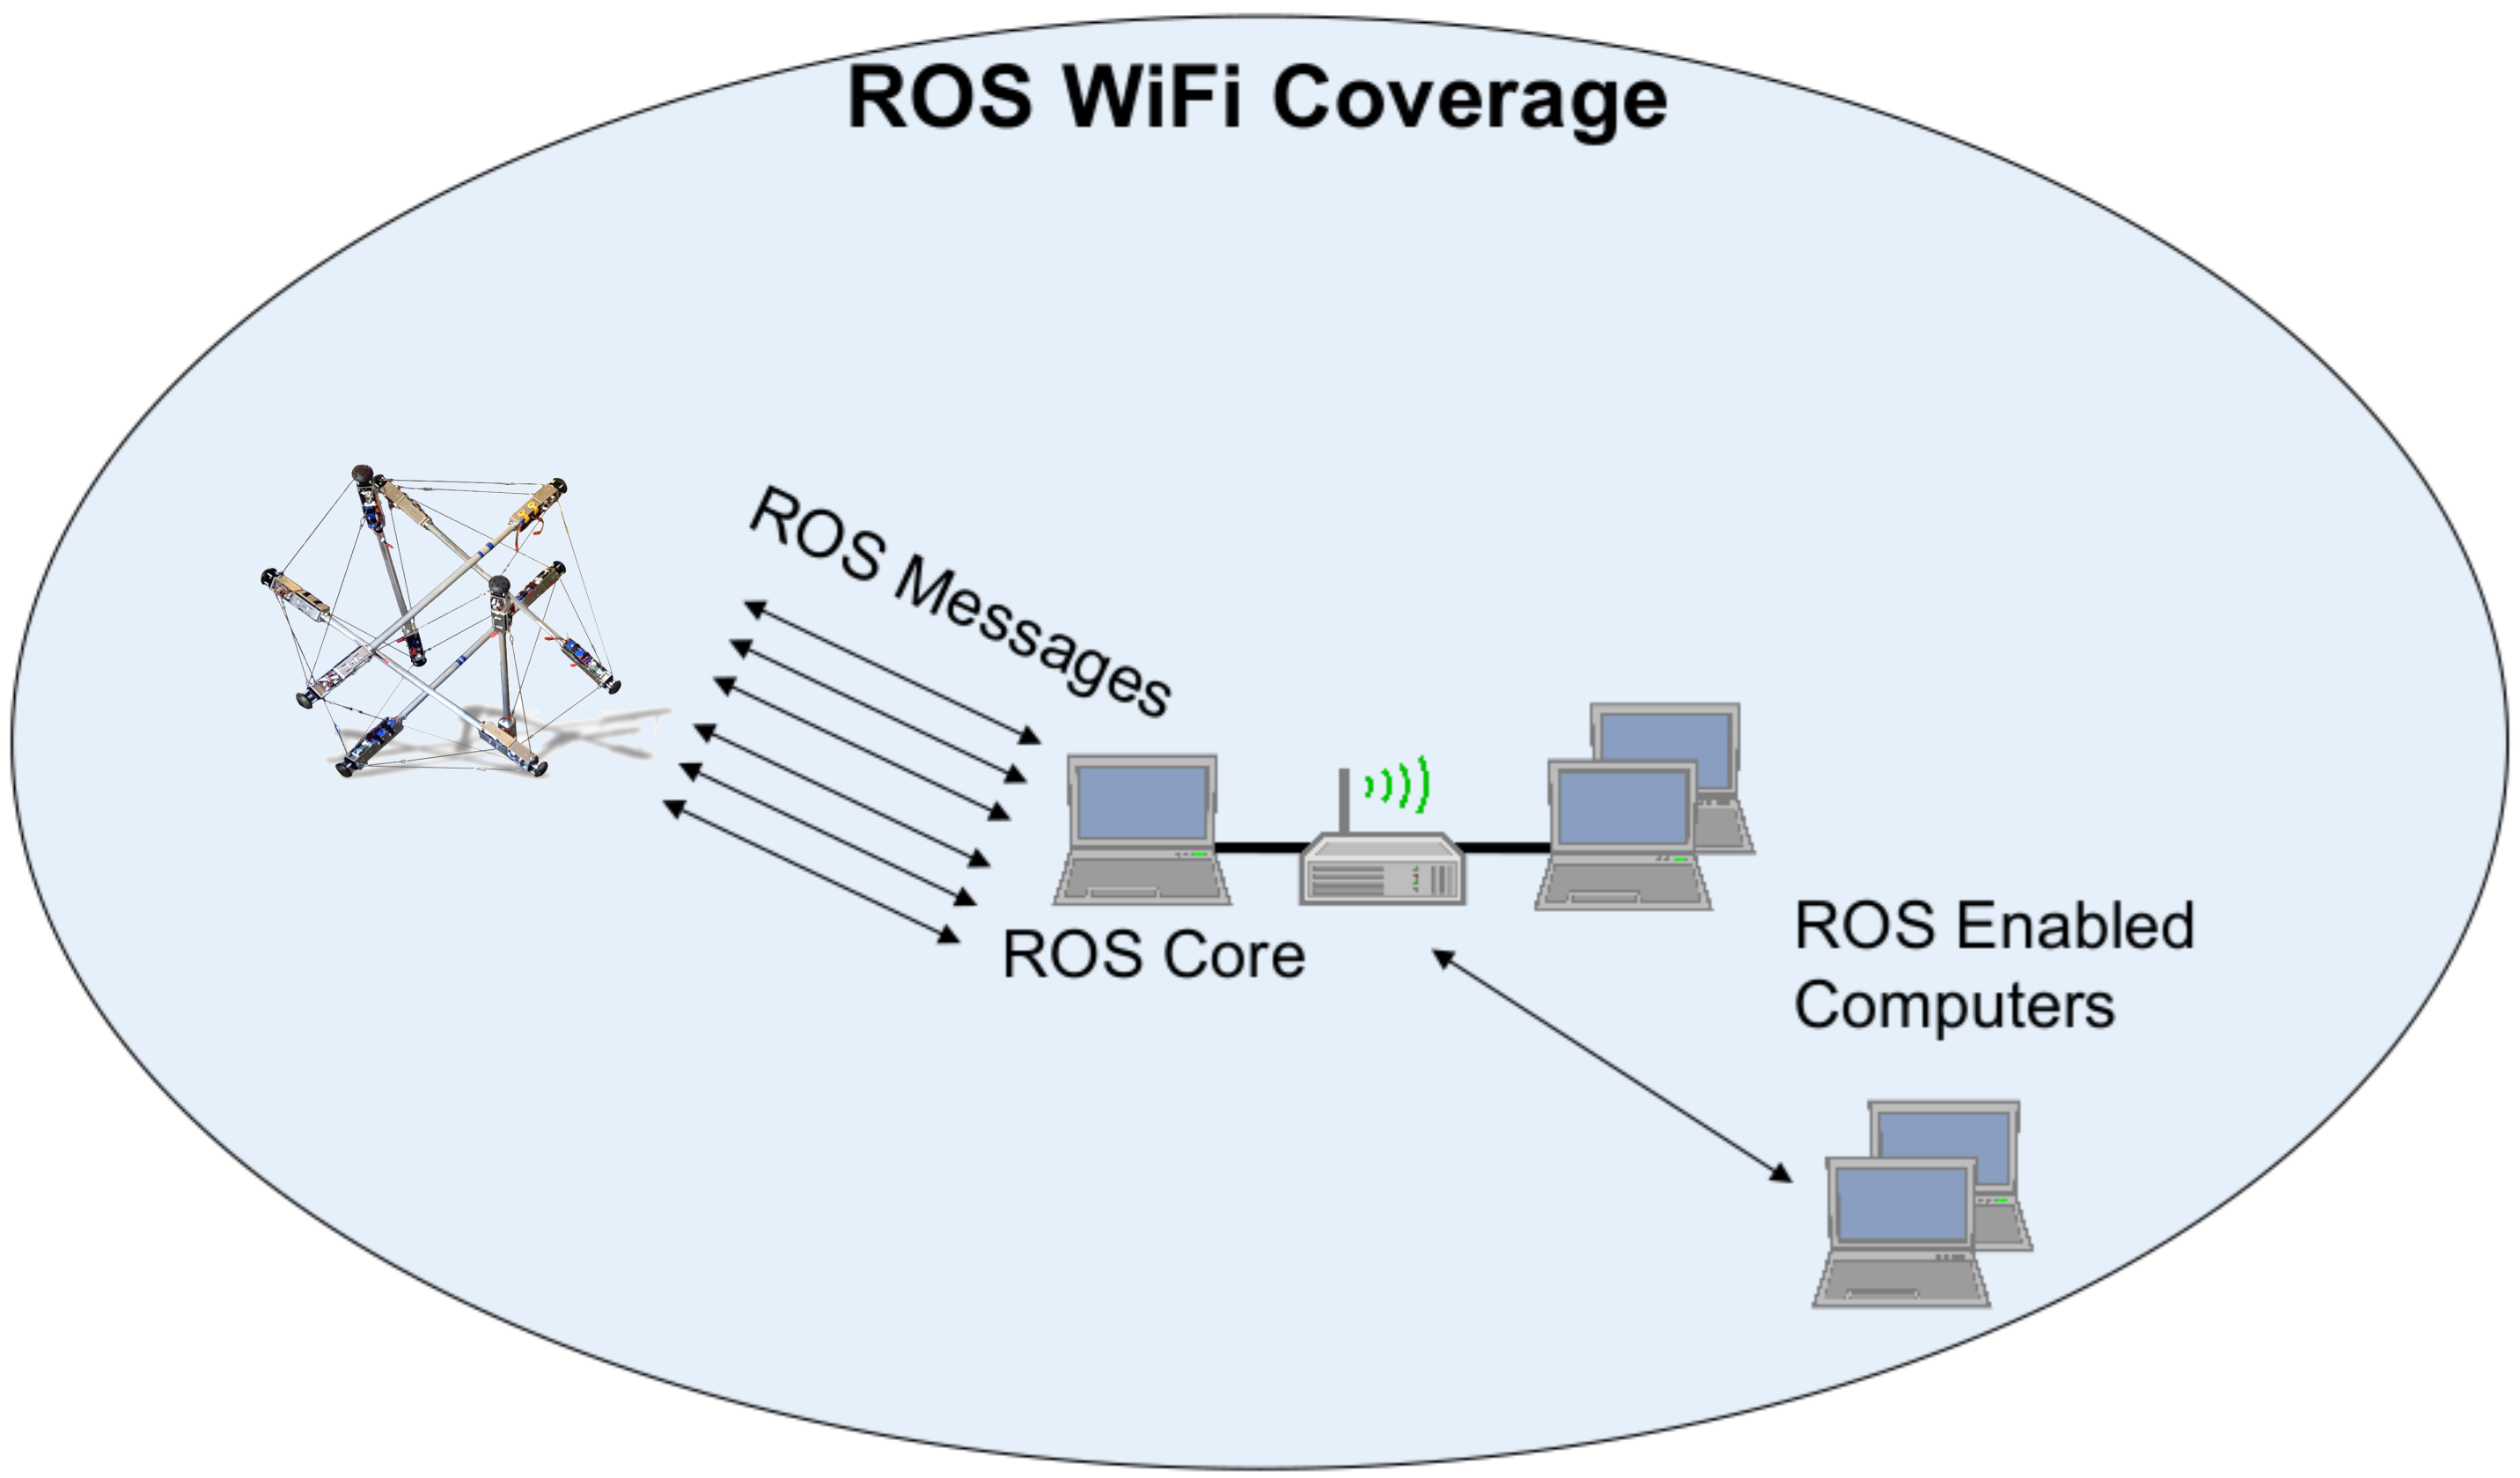
\includegraphics[width=0.8\columnwidth]{tex/img/ROS_Wireless}
      \caption{A simplified representation of how messages are passed within the \SB{} ROS network.}
      %\vspace{-0.5cm}
      \label{fig:ros_diagram}
\end{figure}

\section{Basic Locomotion}
\label{basic_locomotion}
Using a basic step input to a single motor, \SB{} can perform a simple transition from one face of the icosahedron to another.
Figure \ref{fig:superball_flop_flat} shows an test where a motor retracts a cable, induing a flop.
The idea of this type of simple transition is to deform the base equilateral triangle such that the center of mass "moves" over the triangle's edge.
The robot becomes unstable and gravity pulls the system over.
The momentum of the system then rolls the robot through the adjacent isosceles triangle to the next equilateral triangle.
In this test, the motor retraction was preset and experimentally derived earlier.

\begin{figure}[t]
    \centering
    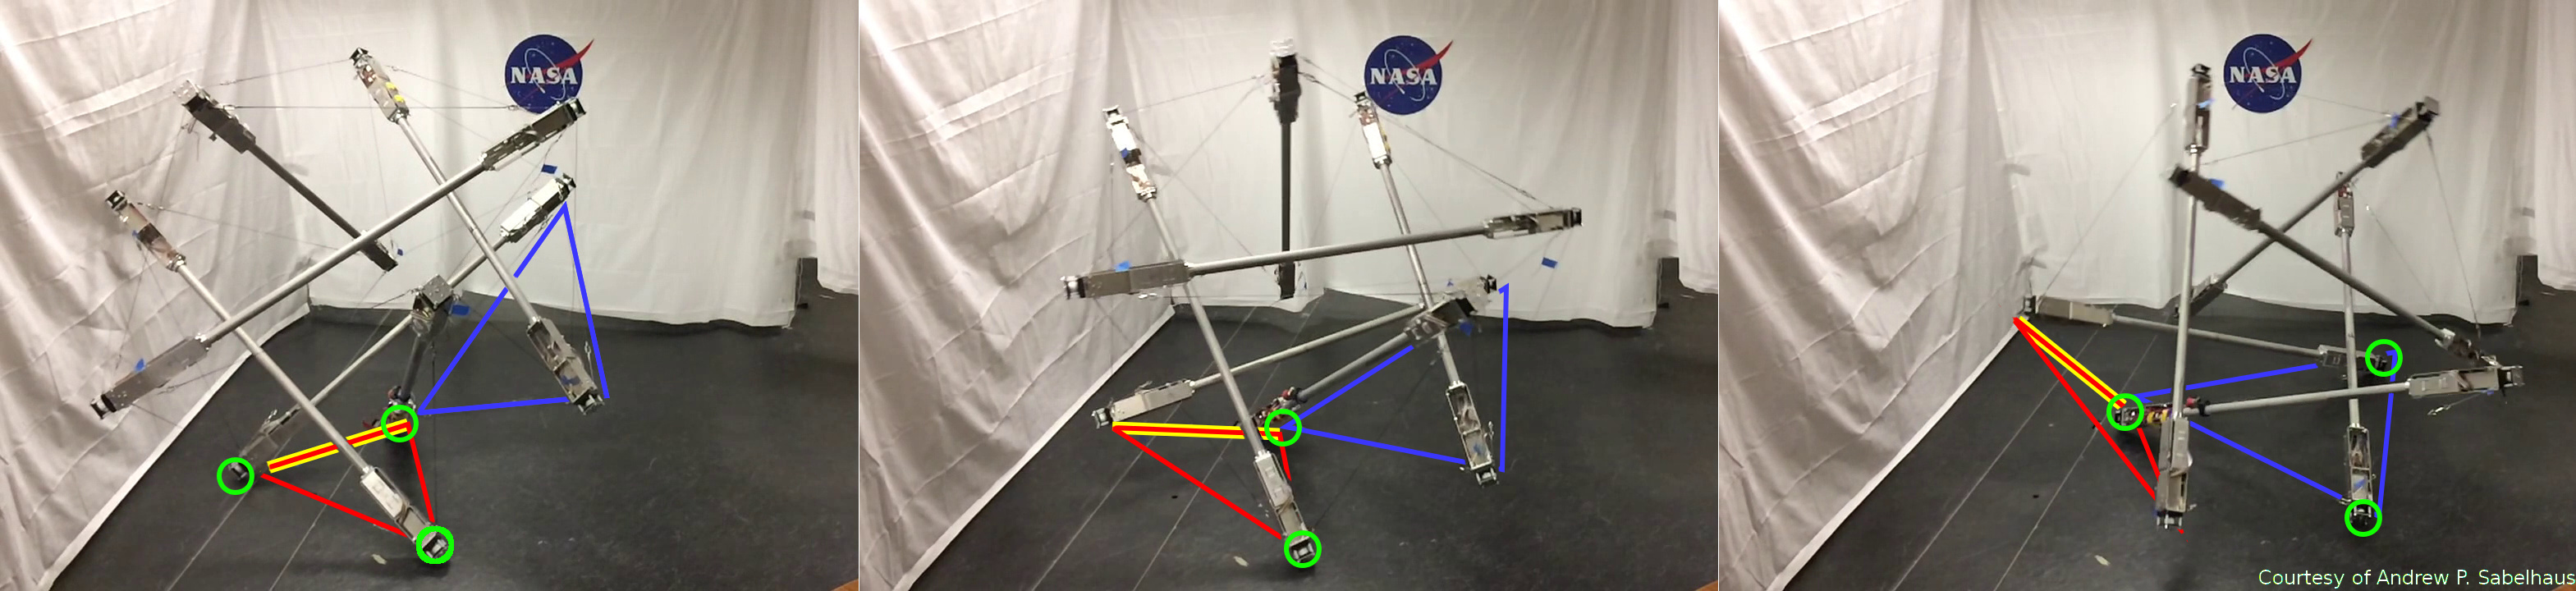
\includegraphics[width=1\linewidth]{tex/img/superball_flop_combined_betterlabels}
    \caption{\SB{} performing a single face-change movement, from one equilateral triangular face to another. The robot begins with all MTRs of the red triangle touching the ground. Then, \SB{} retracts the yellow-highlighted cable on the red triangle, inducing movement. Frame 2 shows \SB{} halfway through the movement with only two points of contact on the ground. Finally, frame 3 shows \SB{} at the end, with all 3 points of the blue triangle in ground contact.}
    \label{fig:superball_flop_flat}
\end{figure}
